\documentclass[12pt]{article} % use larger type; default would be 10pt

%packages
\usepackage[utf8]{inputenc} % set input encoding (not needed with XeLaTeX)
\usepackage{fancyhdr}
\usepackage{float}
\usepackage{geometry}
\usepackage{ulem}
\usepackage{soul}
\usepackage{color}
\usepackage{graphicx}
\usepackage{hyperref}
\usepackage{array}
\usepackage{caption}
\usepackage{titling}
\usepackage{enumerate} 
\usepackage[dvipsnames]{xcolor}
\usepackage{amsmath}
\usepackage{amssymb}
\usepackage[compact]{titlesec}


 %put box around figure captions
\makeatletter
\long\def\@makecaption#1#2{%
  \vskip\abovecaptionskip
  \sbox\@tempboxa{\fbox{#1: #2}}%
  \ifdim \wd\@tempboxa >\hsize
    \fbox{\parbox{\dimexpr\linewidth-2\fboxsep-2\fboxrule}{#1: #2}}\par
  \else
    \global \@minipagefalse
    \hb@xt@\hsize{\hfil\box\@tempboxa\hfil}%
  \fi
  \vskip\belowcaptionskip}
\makeatother

%reduce space between 
\titlespacing{\section}{0pt}{*1}{*0}
\titlespacing{\subsection}{0pt}{*1}{*0}
\titlespacing{\subsubsection}{0pt}{*0}{*0}


%no indent and modify distance between paragraphs
\setlength\parindent{0pt}
\setlength\parskip{12pt}

%set margins and line spacing
\geometry{margin=1in}
\linespread{1.2}
\geometry{letterpaper}

%math operators
\DeclareMathOperator{\E}{\mathbb{E}}

%set up header and page numbering
\pagestyle{fancy}
\lhead{CS 155 Set 5}
\rhead{Timothy Liu}
\pagenumbering{arabic}



\title{CS155 Set 5}
\author{Timothy Liu}

\begin{document}


\maketitle

\newpage

\section{Problem 1}
\subsection{Problem A}

In SVD, $X = U\Sigma V^T$
$$XX^T = (U\Sigma V^T)(U \Sigma V^T)^T = U\Sigma V^T V \Sigma U^T = U \Sigma ^2 U^T$$

and the matrix U matches the principal components in PCA $XX^T = U\Lambda U^T$

The eigenvalues of $XX^T$ are the diagonals of $\Lambda$. The singular values of X in $\Sigma$ are the square root of the eigenvalues along the diagonal of $\Lambda$.

\subsection{Problem B}
The eigenvalues of the PCA of X corresponds to the variance along the corresponding eigenvector. Variances are non-negative, which is why the eigenvalues are also non-negative. Additionally, $\Lambda$ is the square of $\Sigma$ and the square of real numbers are positive. 

\subsection{Problem C}

$$Tr(AB) = \sum_{i = 1}^N (AB)_{ii}$$
The trace can be re-expressed as the sum of the dot product of the $i$th row of A and the $i$th column of B.
$$Tr(AB) = \sum_{i = 0}^{N-1} \sum_{j=0} ^{N-1} A_{ij} \cdot B_{ji} $$

For two matrices we can cyclically permute and have the same result when we take the dot products. To add a third matrix, we take AB as one matrix and are allowed to permute AB and C. This is equivalent to a cyclic permutation.

\subsection{Problem D}
To represent an $N \times N$ with SVD, we need $2 \times N \times k + k$ values. The first term corresponds to the elements of $U$ and $V$ and the second term corresponds to the diagonals of $\Sigma$. Storing the truncated SVD is more efficient for when:
$$k < \frac{N^2}{2N + 1}$$

\subsection{Problem E}
\subsubsection{Part i}
Since $\Sigma$ only has non zero values along the entries $\Sigma_{ii}$ the part of $\Sigma$ that is missing from $\Sigma '$ is all zeros. Multiplying the parts of the matrices that are not removed will result in the same values, and the parts that are missing only yield zeros. Thus $U \Sigma$ yields a $D \times N$ matrix with the same values as $U' \times \Sigma '$ (also $D \times N$).

\subsubsection{Part ii}
For a matrix to be orthogonal, we require $U'U^{'T} = U^{'T}U$. However, since $U'$ is not square the dimensions of these two matrices are not equivalent. $U'U^{T}$ is a $D \times D$ matrix and $U^{T'}U$ is a $N \times N$ matrix.

\subsubsection{Part iii}
We know that $U^T U = I_{D \times D}$. Thus the dot product $U^T_i \cdot U_j = 1$ when $i = j$ and 0 when $i \neq j$ The matrix $U^T U$ is the same matrix, for $i < N$ and thus is also the identity matrix.

This is not true for $U'U^{'T}$. Consider the following counterexample:
\begin{figure}[H]
	\makebox[\textwidth][c]{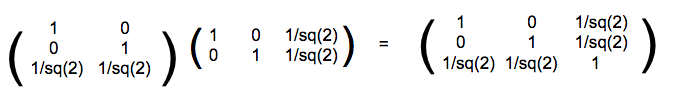
\includegraphics[width=5in]{1e.png}}
	\vspace{-10mm}
\end{figure}


\subsection{Problem F}
\subsubsection{Part i}
We must show that the pseudo-inverse $\Sigma^{+} = \Sigma^{-1}$. We know that $\Sigma$ is a diagonal matrix, and since it is invertible it must also be a square matrix. The inverse of a diagonal square matrix is identical to the original matrix with each non-zero term along the diagonal inverted. Zero terms along the diagonal remain zero. This is identical to the definition we gave in lecture, meaning that $\Sigma^{-1} = \Sigma ^ {+}$.

\subsubsection{Part ii}
We know that $X$ can be decomposed into $U\Sigma V^T$. Substituting into the expression for the pseudo-inverse gives us:

$$X^{+'} = (X^T X)^{-1}X^T$$
$$X^{+'} = ((U\Sigma V^T)^T U\Sigma V^T)^{-1}(U\Sigma V^T)^T$$
$$X^{+'} = (V\Sigma U^T U\Sigma V^T)^{-1}(U\Sigma V^T)^T$$
$$X^{+'} = (V \Sigma^2 V^T)^{-1}(U\Sigma V^T)^T$$
$$X^{+'} = (V \Sigma^2 V^T)^{-1}V\Sigma U^T$$
$$X^{+'} = V^{T ^ {-1}} \Sigma^{2^{-1}} V^{-1}V\Sigma U^T$$
$$X^{+'} = V^{T ^ {-1}} \Sigma^{2^{-1}} \Sigma U^T$$
$$X^{+'} = V^{T ^ {-1}} \Sigma^{-1}  U^T$$

Since V is a orthogonal matrix and $V^T = V^{-1}$:
$$X^{+'} = V^{T ^ {T}} \Sigma^{-1}  U^T$$
$$X^{+'} = V \Sigma^{-1}  U^T$$

\subsubsection{Part iii}
The technique in part ii is less stable. The technique requires squaring $\Sigma$ which makes it more sensitive to errors rather than just $\Sigma$. Additionally the least squares term has multiple X terms, allowing for errors in X to propagate.

\section{Problem 2}

\subsection{Problem A}
%u_i
\underline{Gradient $u_i$}
$$\partial_{u_i}\bigg(\frac{\lambda}{2}(||U||_F^2 + ||V||_F^2) + \frac{1}{2}\sum_{i, j} (y_{ij} - u_i^Tv_j)^2\bigg)$$
%
$$\partial_{u_i}\bigg(\frac{\lambda}{2}(||U||_F^2 + ||V||_F^2)\bigg) + \partial_{u_i}\bigg(\frac{1}{2}\sum_{i, j} (y_{ij} - u_i^Tv_j)^2\bigg)$$
%
$$\partial_{u_i}\bigg(\frac{\lambda}{2}(||U||_F^2 + ||V||_F^2)\bigg) -\sum_{j}v_j (y_{ij} - u_i^Tv_j)$$
%
$$\frac{\lambda}{2}\partial{u_i}\sqrt{\sum_{i, j} u_{i,j}^2} -v_j\sum_{j} (y_{ij} - u_i^Tv_j)$$
%
$$\lambda u_i -\sum_{j} v_j(y_{ij} - u_i^Tv_j)$$

%v_j
\underline{Gradient $v_j$}
%
$$\partial_{v_j}\bigg(\frac{\lambda}{2}(||U||_F^2 + ||V||_F^2) + \frac{1}{2}\sum_{i, j} (y_{ij} - u_i^Tv_j)^2\bigg)$$
%
$$\partial_{v_j}\bigg(\frac{\lambda}{2}(||U||_F^2 + ||V||_F^2)\bigg) + \partial_{v_j}\bigg(\frac{1}{2}\sum_{i, j} (y_{ij} - u_i^Tv_j)^2\bigg)$$
%
$$\partial_{v_j}\bigg(\frac{\lambda}{2}(||U||_F^2 + ||V||_F^2)\bigg) -\sum_{i, j} u_i^T (y_{ij} - u_i^Tv_j)$$
%
$$\frac{\lambda}{2}\partial{u_i}\sqrt{\sum_{i, j} v_{i,j}^2} -v_j\sum_{j} (y_{ij} - u_i^Tv_j)$$
%
$$\lambda v_j - \sum_{j} v_j (y_{ij} - u_i^Tv_j)$$




\subsection{Problem B}

%u_i
\underline{Optimal $u_i$}

$$\partial_{u_i}\bigg(\frac{\lambda}{2}(||U||_F^2 + ||V||_F^2) + \frac{1}{2}\sum_{i, j} (y_{ij} - u_i^Tv_j)^2\bigg) = 0$$
$$\lambda u_i -\sum_{j} v_j(y_{ij} - u_i^Tv_j) = 0$$
$$\lambda u_i -\sum_{j} v_j y_{ij} + \sum_{j} u_i^Tv_j v_j^T = 0$$
$$\lambda u_i + \sum_{j} u_i^T v_j v_j^T= \sum_{j} v_j y_{ij}$$
$$u_i \bigg(\lambda I_K + \sum_{j} v_j v_j^T\bigg)= \sum_{j} v_j y_{ij}$$
$$u_i = \bigg(\lambda I_K + \sum_{j} v_j v_j^T\bigg)^{-1} \sum_{j} v_j y_{ij}$$
%v_j
\underline{Optimal $v_j$}
$$\partial_{v_j}\bigg(\frac{\lambda}{2}(||U||_F^2 + ||V||_F^2) + \frac{1}{2}\sum_{i, j} (y_{ij} - u_i^Tv_j)^2\bigg) = 0$$
$$\lambda v_j -\sum_{j} u_i^T(y_{ij} - u_i^Tv_j) = 0$$
$$\lambda v_j -\sum_{j} u_i^T y_{ij} + \sum_{j} u_i^Tu_i v_j^T = 0$$
$$\lambda v_j + \sum_{j} v_j u_i u_i^T= \sum_{j} u_i y_{ij}$$
$$v_j \bigg(\lambda I_K + \sum_{j} u_i u_i^T\bigg)= \sum_{j} u_i y_{ij}$$
$$v_j = \bigg(\lambda I_K + \sum_{j} u_i u_i^T\bigg)^{-1} \sum_{j} u_i y_{ij}$$


\subsection{Problem C}
See attached code.

\subsection{Problem D}

\begin{figure}[H]
	\makebox[\textwidth][c]{\includegraphics[width=5in]{2D.png}}
	\vspace{-10mm}
	\caption{Performance of latent factor model as function of K}
\end{figure}

As the number of parameters K increases, the in sample error decreases because the model fit is improving. However, the out of sample error increases because of overfitting.

\subsection{Problem E}

\begin{figure}[H]
	\makebox[\textwidth][c]{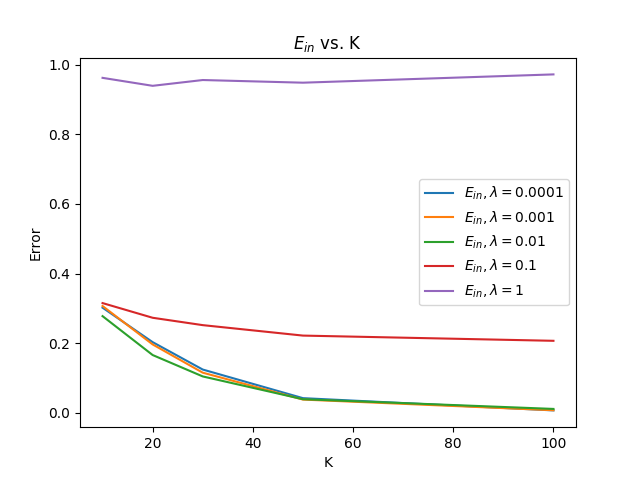
\includegraphics[width=5in]{2e_ein.png}}
	\vspace{-10mm}
	\caption{In sample performance of latent factor model with regularization}
\end{figure}

\begin{figure}[H]
	\makebox[\textwidth][c]{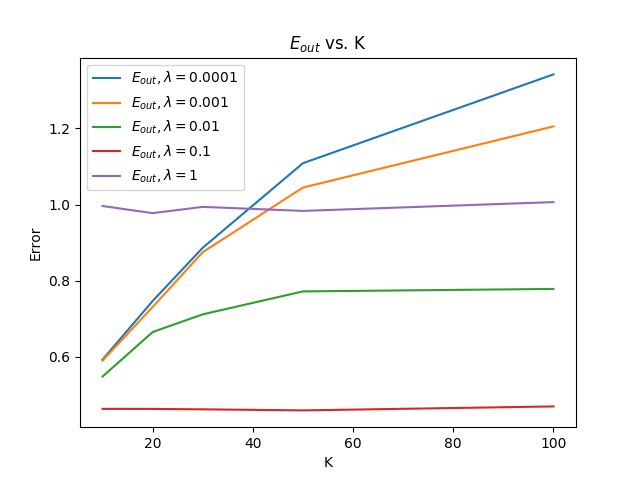
\includegraphics[width=5in]{2e_eout.png}}
	\vspace{-10mm}
	\caption{Out of sample performance of latent factor model with regularization}
\end{figure}

Increasing the amount of regularization smooths the out of sample training error as the number of latent factors increases. In sample, regularization slightly worsens the performance but the error increases as lambda goes up to 0.1 and 1. Out of sample, $\lambda = 1$ has the least error. The error has a minimum around K = 50.

\section{Problem 3}
\subsection{Problem A}
Since we need a gradient for each pair of words, the number of gradients scales by $O(W^2)$. We also need a gradient along each dimension in the embedding, so the total number of gradients scales by $O(W^2 D)$.

\subsection{Problem B}

\begin{figure}[H]
	\makebox[\textwidth][c]{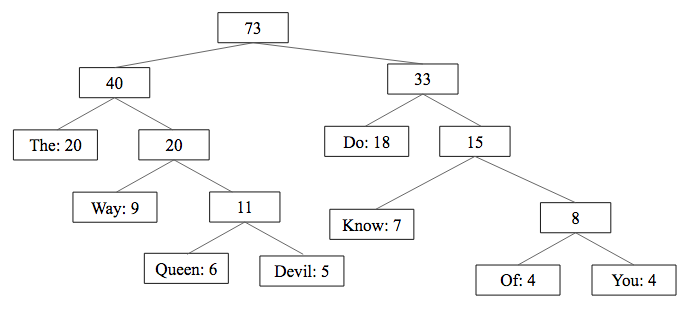
\includegraphics[width=5in]{huffman.png}}
	\vspace{-10mm}
	\caption{Huffman Tree.}
\end{figure}

\begin{figure}[H]
	\makebox[\textwidth][c]{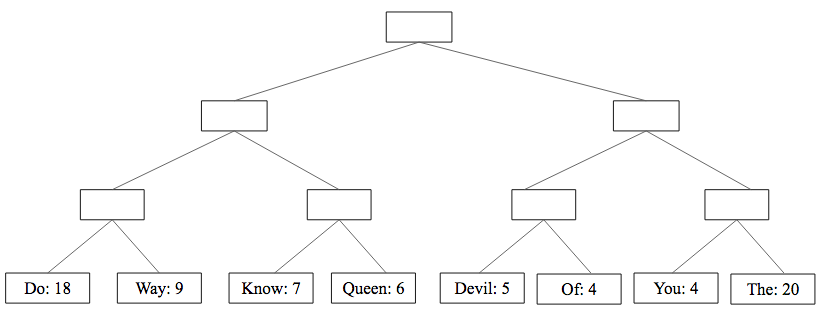
\includegraphics[width=5in]{binary.png}}
	\vspace{-10mm}
	\caption{Binary Tree.}
\end{figure}

Average word length for Huffman:
$$2 * \frac{18}{73} + 3 * \frac{9}{73} + 3 * \frac{7}{93} + 2 * \frac{20}{73} + 4 * \frac{6}{73} + 4 * \frac{5}{73} + 4 * \frac{4}{73} + 4 * \frac{4}{73}$$

$$ = 2.68 $$

Average word length for binary: 3

\subsection{Problem C}
As the number of dimensions increases, the training objective will increase. Having too many dimensions will lead to overfitting.

\subsection{Problem D}
See attached code.

\subsection{Problem E}
\subsubsection{Part i}
The weight matrix for the hidden layers is (308, 10) which maps to 308 words to 10 hidden units.

\subsubsection{Part ii}
The weight matrix for the output layers is (10, 308) which corresponds to the 10 hidden layers to 308 classifications.

\subsubsection{Part iii}

Pair(green, thank), Similarity: 0.98398983  \\
Pair(thank, green), Similarity: 0.98398983  \\
Pair(goat, boat), Similarity: 0.98270833  \\
Pair(boat, goat), Similarity: 0.98270833  \\
Pair(gone, tomorrow), Similarity: 0.9774943  \\
Pair(tomorrow, gone), Similarity: 0.9774943  \\
Pair(eight, nine), Similarity: 0.97380567  \\
Pair(nine, eight), Similarity: 0.97380567  \\
Pair(today, tomorrow), Similarity: 0.9718245  \\
Pair(may, samiam), Similarity: 0.97140914  \\
Pair(samiam, may), Similarity: 0.97140914  \\
Pair(wire, goodbye), Similarity: 0.97121143  \\
Pair(goodbye, wire), Similarity: 0.97121143  \\
Pair(fox, goat), Similarity: 0.9671794  \\
Pair(shoe, cold), Similarity: 0.96702147  \\
Pair(cold, shoe), Similarity: 0.96702147  \\
Pair(heads, grows), Similarity: 0.96493155  \\
Pair(grows, heads), Similarity: 0.96493155  \\
Pair(anywhere, samiam), Similarity: 0.9638241  \\
Pair(rain, goat), Similarity: 0.95803976  \\
Pair(off, shoe), Similarity: 0.95780945  \\
Pair(seven, ten), Similarity: 0.9576886  \\
Pair(ten, seven), Similarity: 0.9576886  \\
Pair(do, green), Similarity: 0.95573854  \\
Pair(box, anywhere), Similarity: 0.95573425  \\
Pair(or, anywhere), Similarity: 0.9549918  \\
Pair(five, seven), Similarity: 0.95334554  \\
Pair(with, box), Similarity: 0.9524708  \\
Pair(mouse, fox), Similarity: 0.95199776  \\
Pair(would, goat), Similarity: 0.9489787  \\

The pairs of words are often reciprocal pairs. The word pairs are also ones that appear frequently together in Dr. Seuss or are words that rhyme.



\end{document}










